\documentclass{article}
\usepackage{fullpage}
\usepackage{graphicx}
\usepackage{url}
\begin{document}

\title{Pmod On Nexys3 Controller and DUT}

\maketitle

\begin{figure}[ht]
  \begin{center}
    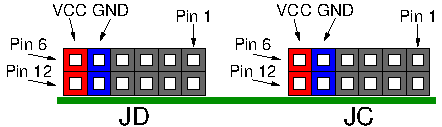
\includegraphics[scale=1]{figures/pmod_connector}
    \caption{Pmod Connectors as Viewed from Front}
  \end{center}
\end{figure}

\begin{table}[ht]
  \begin{center}
    \caption{Pin Configuration on Nexys3}
    \begin{tabular}{llll|llll}
      Pin  & LOC & Net         & Comment & Pin  & LOC & Net        & Comment \\ \hline
       JC1 & H3  & DUTClock    & GCLK20  &  JD1 & G11 & reset      & \\
       JC2 & L7  & src\_ready  &         &  JD2 & F10 & dst\_ready & \\
       JC3 & K6  & datain[3]   &         &  JD3 & F11 & dataout[3] & \\
       JC4 & G3  & datain[1]   &         &  JD4 & E11 & dataout[1] & \\
       JC5 &	 & 			   & GND     &  JD5 &     & GND        & \\
       JC7 & G1  & src\_read   &         &  JD7 & D12 &            &\\
       JC8 & J1  & 			   &         &  JD8 & C12 & dst\_write & \\
       JC9 & J6  & datain[2]   &         &  JD9 & F12 & dataout[2] & \\
      JC10 & F2  & datain[0]   &         & JD10 & E12 & dataout[0] & \\
    \end{tabular}
  \end{center}
\end{table}

\begin{figure}[ht]
  \begin{center}
    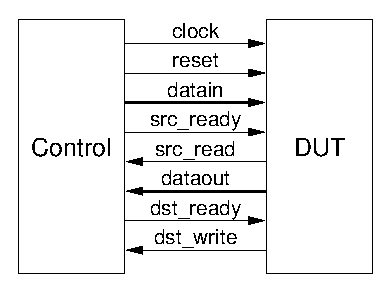
\includegraphics[scale=1]{figures/ctrl-dut_connections}
    \caption{Connections between Control and DUT}
  \end{center}
\end{figure}

\end{document}
